% Metódy inžinierskej práce

\documentclass[10pt,twoside,slovak,a4paper]{article}

\usepackage[slovak]{babel}
%\usepackage[T1]{fontenc}
\usepackage[IL2]{fontenc} % lepšia sadzba písmena Ľ než v T1
\usepackage[utf8]{inputenc}
\usepackage{graphicx}
\usepackage{url} % príkaz \url na formátovanie URL
\usepackage{hyperref} % odkazy v texte budú aktívne (pri niektorých triedach dokumentov spôsobuje posun textu)

\usepackage{cite}
%\usepackage{times}

\pagestyle{headings}

\title{Model algoritmu na rozpoznávanie tvárí\thanks{Semestrálny projekt v predmete Metódy inžinierskej práce, ak. rok 2021/22, vedenie: Ing. Ján Lučanský}} % meno a priezvisko vyučujúceho na cvičeniach

\author{Viktor Repka\\[2pt]
	{\small Slovenská technická univerzita v Bratislave}\\
	{\small Fakulta informatiky a informačných technológií}\\
	{\small \texttt{xrepkav@stuba.sk}}
	}

\date{\small 5. november 2021} % upravte



\begin{document}

\maketitle

\begin{abstract}

Tento článok sa venuje strojovému rozoznávaniu tváre. Chcel by som v ňom priblížiť proces potrebný pre priradenie identity k vstupu v podobe fotky tváre so zameraním na predspracovanie a normalizáciu vstupného obrazu. Budem sa venovať hlavne problematike rozpoznávania na základe jednej vstupnej vzorky. 
\end{abstract}

\pagebreak

\section{Úvod}

Štandarne využívaný postup pri spoznávaní tvare vyžaduje veľké množstvo vstupných dát, dát uložených v databáze a veľkú výpočtovú silu. Ak by sa využíval len jeden vstupný obraz a v databázach by postačoval menší objem dát pre pre každú uloženú osobu, znížili by sa tým náklady na prevádzku. 
Zníženie množtva vstupných dát spôsobí extrakciu menšieho množstva pŕiznakov, čo vedie k menšej úspešnosti rozoznávania. Tento efekt sa ale dá zmierniť niektorými postupmi, ktoré priblížim v ďaších kapitolách. 

\section{Ako funguje rozpoznávanie tvárí}

\begin{figure*}[tbh]
\centering
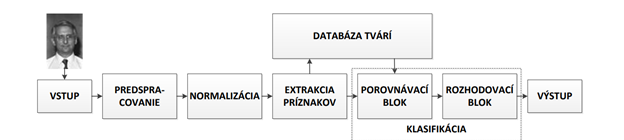
\includegraphics[width=\textwidth]{Picture3.png}
\caption{Schematické znázornenie zovšeobecneného modelu rozpoznavania tvárí.\cite{Ban1}}
\label{f:facerecmod}
%Aj text môže byť prezentovaný ako obrázok. Stane sa z neho označný plávajúci objekt. Po vytvorení diagramu zrušte znak \texttt{\%} pred príkazom \verb|%\includegraphics| označte tento riadok ako komentár (tiež pomocou znaku \texttt{\%}).
%\caption{Rozhodujúci argument.}
%\label{f:rozhod}
\end{figure*}



Rozpoznávanie tváre pozostáva z viacerých na seba nadväzujúcich procesov, ktoré je možné
charakterizovať vo viacerých blokoch. Z týchto blokov je možné zostaviť model
rozpoznávania tvárí (Obr.  \ref{f:facerecmod}).

Vstupný blok zahŕňa zosnímanie tváre pomocou kamery. Zachytený obraz je následne
predspracovaný. Tento krok môže zahŕňať odstránenie šumu, detekovanie tváre, alebo iné
špeciálne upravy.

V bloku normalizácie sa upravujú vlastnosti ako natočenie tváre a úprava jej veľkosti.
Nasleduje extrakcia príznakov. Príznaky sú charakteristiky s najväčšou informačnou hodnotou.
Extrahované príznaky sa porovnajú s výsledkami uloženými v databáze.

V rozhodovacom bloku sa na základe predošlých výpočtov určí identita vstupnej osoby, za
predpokladu, že sa daná osoba nachádza v prehľadávanej databáze.
Výsledky (identita osoby alebo záznam) sa následne zobrazia na výstupnom zariadení.\cite{Ban1}

%Motivujte čitateľa a vysvetlite, o čom píšete. Úvod sa väčšinou nedelí na časti.

%Uveďte explicitne štruktúru článku. Tu je nejaký príklad.
%Základný problém, ktorý bol naznačený v úvode, je podrobnejšie vysvetlený v časti~\ref{nejaka}.
%Dôležité súvislosti sú uvedené v častiach~\ref{dolezita} a~\ref{dolezitejsia}.
%Záverečné poznámky prináša časť~\ref{zaver}.





\section{Úprava vstupného obrazu} \label{nejaka}

%Z obr.~\ref{f:rozhod} je všetko jasné. 


\subsection{2DPCA (two-dimensional PCA)} \label{2DPCA}



V prípade nedostatku snímkov pre porovnanie je možné vygenerovaťnové snímky pomocou úpravy jasu a kontrastu alebo pridaním šum (Gaussian blur). Vygenerované snímky sú novými reprezentáciami snímku pôvodného a zvyšujú pravdepodobnosť správnej identifikácie. V porovnaní s tridičnou metódou (eigenface method) prejavuje metóda 2DPCA zvýšenie úspešnosti až o 10\texttt{\%}.
Keď bola testovaná na vzorke 137 tvárí zoskenovaných z identifikačných kariet bolo zaznamenaná chybovosť bola len 1,32\texttt{\%}.\cite{article1}

\begin{figure*}[tbh]
\centering
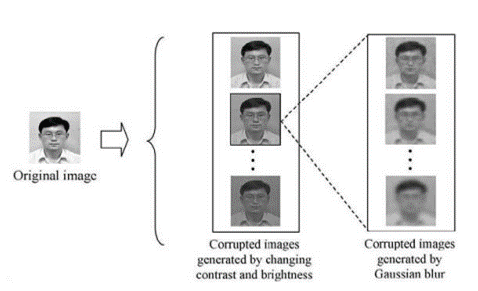
\includegraphics[width=\textwidth]{Picture1.png}
\caption{Syntetizovanie nových vzoriek pomocou šumu (niose model).\cite{article1}}
\label{f:noise}
\end{figure*}

\subsection{Generovanie alternatívnych pohľadov(Generate novel views)} \label{ina:nejake}

\begin{figure*}[tbh]
\centering
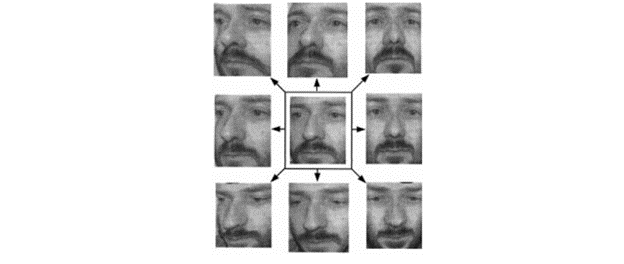
\includegraphics[width=\textwidth]{Picture2.png}
\caption{Pôvodný obraz (v strede) obklopený obrazmi generovanými metódou paralelnej deformácie.\cite{article1}}
\label{f:multiangle}
\end{figure*}

Tento prístup umožnuje vyvoriť snímky s iným uhlom pohľadu ako tým na pôvodnej snímke. Aby bol tento proces možný je najprv potrebné vycvičiť software na dostatočnej vzorke snímok, ktoré obsahujú viac snímkov jednej osoby.\cite{article1}


%\subsection{EMPTY)} \label{EMPTY}
%Niekedy treba uviesť zoznam:

%\begin{itemize}
%\item jedna vec
%\item druhá vec
%	\begin{itemize}
%	\item x
%	\item y
%	\end{itemize}
%\end{itemize}

%Ten istý zoznam, len číslovaný:

%\begin{enumerate}
%\item jedna vec
%\item druhá vec
%	\begin{enumerate}
%	\item x
%	\item y
%	\end{enumerate}
%\end{enumerate}


%\subsection{Ešte nejaké vysvetlenie} \label{ina:este}

%\paragraph{Veľmi dôležitá poznámka.}
%Niekedy je potrebné nadpisom označiť odsek. Text pokračuje hneď za nadpisom.



%\section{Dôležitá časť} \label{dolezita}




%\section{Ešte dôležitejšia časť} \label{dolezitejsia}




%\section{Záver} \label{zaver} % prípadne iný variant názvu



%\acknowledgement{Ak niekomu chcete poďakovať\ldots}


% týmto sa generuje zoznam literatúry z obsahu súboru literatura.bib podľa toho, na čo sa v článku odkazujete
\bibliography{literatura}
\bibliographystyle{plain} % prípadne alpha, abbrv alebo hociktorý iný
\end{document}
